\documentclass[border=10pt]{standalone}
\usepackage{tikz}
\usetikzlibrary{arrows.meta}
\begin{document}
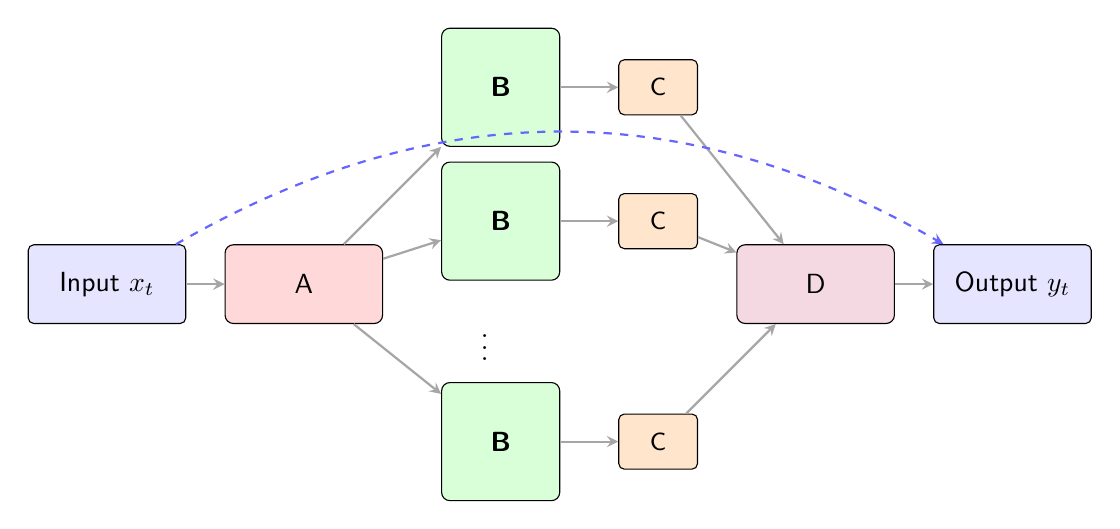
\begin{tikzpicture}[
    node distance=1.5cm,
    box/.style={rectangle, draw, rounded corners=2pt, fill=blue!10, minimum width=2cm, minimum height=1cm, font=\sffamily},
    expert/.style={rectangle, draw, rounded corners=3pt, fill=green!15, minimum width=1.5cm, minimum height=1.5cm, font=\sffamily\bfseries},
    router/.style={rectangle, draw, rounded corners=3pt, fill=red!15, minimum width=2cm, minimum height=1cm, font=\sffamily},
    combiner/.style={rectangle, draw, rounded corners=3pt, fill=purple!15, minimum width=2cm, minimum height=1cm, font=\sffamily},
    weight/.style={rectangle, draw, rounded corners=2pt, fill=orange!20, minimum width=1cm, minimum height=0.7cm, font=\sffamily\small},
    thick_arrow/.style={-stealth, thick, draw=gray!70},
    skip_arrow/.style={-stealth, thick, dashed, draw=blue!60},
    label/.style={font=\sffamily\small}
]
    % Input
    \node[box] (input) at (0,0) {Input $x_t$};
    % Router
    \node[router] (router) at (2.5,0) {A};
    % Experts
    \node[expert] (e1) at (5,2.5) {B};
    \node[expert] (e2) at (5,0.8) {B};
    \node[text width=0.5cm] (dots) at (5,-0.7) {$\vdots$};
    \node[expert] (en) at (5,-2) {B};
    % Weights
    \node[weight] (w1) at (7,2.5) {C};
    \node[weight] (w2) at (7,0.8) {C};
    \node[weight] (wn) at (7,-2) {C};
    % Output combining
    \node[combiner] (combine) at (9,0) {D};
    % Final output
    \node[box] (output) at (11.5,0) {Output $y_t$};
    % Arrows
    \draw[thick_arrow] (input) -- (router);
    \draw[thick_arrow] (router) -- (e1);
    \draw[thick_arrow] (router) -- (e2);
    \draw[thick_arrow] (router) -- (en);
    \draw[thick_arrow] (e1) -- (w1);
    \draw[thick_arrow] (e2) -- (w2);
    \draw[thick_arrow] (en) -- (wn);
    \draw[thick_arrow] (w1) -- (combine);
    \draw[thick_arrow] (w2) -- (combine);
    \draw[thick_arrow] (wn) -- (combine);
    \draw[thick_arrow] (combine) -- (output);
    % Skip connection
    \draw[skip_arrow] (input) to[out=30, in=150] (output);
\end{tikzpicture}
\end{document}
